
%(BEGIN_QUESTION)
% Copyright 2007, Tony R. Kuphaldt, released under the Creative Commons Attribution License (v 1.0)
% This means you may do almost anything with this work of mine, so long as you give me proper credit

A business owns a large storage tank which was used to hold water for fire protection.  This tank is equipped with a pressure gauge at the bottom to infer water level.  The face of the gauge reads out in feet of water rather than PSI or some other common pressure unit:

$$\includegraphics[width=15.5cm]{i02949x01.eps}$$

The operation of this level-indicating pressure gauge is quite simple: as the water level changes in the tank, the amount of hydrostatic pressure generated at the bottom changes proportionally.

\vskip 10pt

When the local municipality upgrades the size of the water supply line to the company property, there is no longer a need for the fire-water storage tank.  Not wanting to abandon the tank, a manager at the company decides to use it for gasoline fuel storage instead.  

After emptying the water and re-filling the tank with gasoline, however, they notice a problem with the level-indicating gauge: it no longer reads correctly.  With gasoline in the tank instead of water, the gauge's reading no longer correlates with tape-measure readings of liquid level like it used to.  Instead, the gauge consistently registers low: there is always more gasoline in the tank than the gauge indicates.

Someone at this company asks you to explain what the problem is, because you have studied instrumentation technology.  Describe the nature of the problem in your own words, and propose a solution to this problem that does not involve purchasing any new equipment.

\vskip 20pt \vbox{\hrule \hbox{\strut \vrule{} {\bf Suggestions for Socratic discussion} \vrule} \hrule}

\begin{itemize}
\item{} If there is actually 10 feet of gasoline in the tank, how many feet with the water-calibrated gauge read?
\end{itemize}

\underbar{file i02949}
%(END_QUESTION)





%(BEGIN_ANSWER)

The problem is that gasoline is less dense than water: for the same liquid height in the tank, gasoline generates less hydrostatic pressure than water.  The solution is to re-calibrate the gauge!

\vskip 10pt

Answer to Socratic question: the gauge will register about 6.7 feet of liquid.  The density of gasoline varies between 41 and 43 pounds per cubic foot, so the range of possibilities here for gauge reading is 6.57 feet to 6.89 feet.

%(END_ANSWER)





%(BEGIN_NOTES)


%INDEX% Measurement, level: hydrostatic pressure

%(END_NOTES)


